 \begin{surferPage}{庫默爾四次曲面}
1895年,恩斯特·庫默爾(Ernst Kummer)第一次具體的提出研究$d$次曲面上最大奇異點個數$\mu(d)$的問題。
他證明了$4$次曲面上最大奇異點個數是$16$。隨後,他詳細的研究了具有$16$個奇異點的$4$次曲面。下面是這樣一類漂亮的曲面:
 \[\bigl(x^2+y^2+z^2-\mu^2\bigr)^2 - \lambda
    \,y_0\,y_1\,y_2\,y_3,\]
    其中 $\mu$ 是一個自由參數,
    $\lambda = \frac{3\mu^2-1}{3-\mu^2}$, $y_i$是如下一個四面體的面 {\small
    $y_0=1-z-\sqrt{2}x$, \
    $y_1=1-z+\sqrt{2}x$, \
    $y_2=1+z+\sqrt{2}y$, \
    $y_3=1+z-\sqrt{2}y$}。雖然不是所有的曲面都正好具有$16$個奇異點,但是大部分是具有$16$個奇異點的:

  \begin{center}
    \vspace*{-0.2cm}\hspace*{-0.2cm}
    \begin{tabular}{@{}c@{\,}c@{\,}c@{\,}c@{\,}c@{}}
      \begin{tabular}{@{}c@{}}
        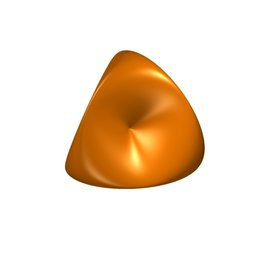
\includegraphics[height=1.4cm]{./../../common/images/kummer_0}
      \end{tabular}
      &
      \begin{tabular}{@{}c@{}}
        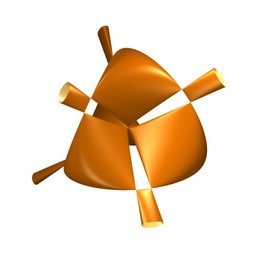
\includegraphics[height=1.4cm]{./../../common/images/kummer_1}
      \end{tabular}
      &
      \begin{tabular}{@{}c@{}}
        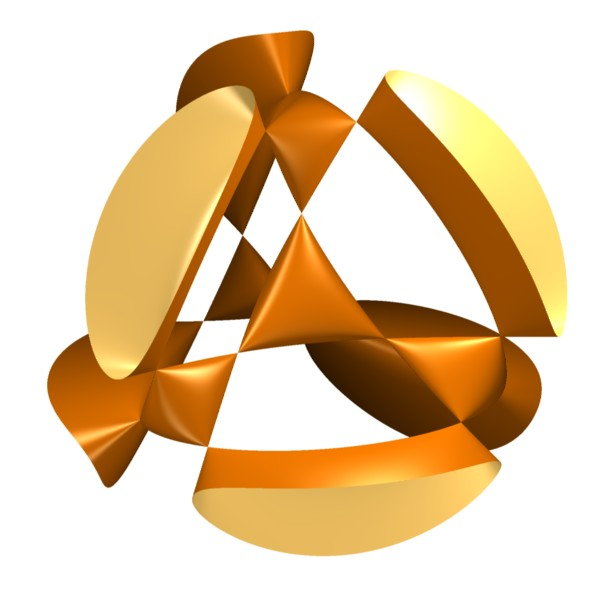
\includegraphics[height=1.4cm]{./../../common/images/kummer_2}
      \end{tabular}
      &
      \begin{tabular}{@{}c@{}}
        
\includegraphics[height=1.4cm]{./../../common/images/kummer_3}
      \end{tabular}
    \end{tabular}
  \end{center}
  \vspace{-0.2cm}
  參數取不同值時,奇異點有可能重合。
\end{surferPage}


